\section{Pomiar wydajności}

Istotnym elementem oceny jakości oprogramowania jest analiza wydajności kluczowych operacji. W przypadku komponentu renderującego, jedną z najbardziej czasochłonnych operacji jest ładowanie trójwymiarowych modeli z plików w formacie OBJ. W niniejszym rozdziale przedstawiono metodykę pomiaru oraz wyniki analizy wydajności funkcji odpowiedzialnej za wczytywanie geometrii.

\subsection{Metodyka pomiaru}

Do przeprowadzenia pomiarów wykorzystano bibliotekę Google Benchmark, która umożliwia precyzyjne i powtarzalne mierzenie czasu wykonania funkcji w języku C++. Wyniki zostały zwizualizowane przy pomocy biblioteki Matplot++. Każdy test został wykonany dziesięciokrotnie, co pozwoliło na obliczenie miar statystycznych: średniej arytmetycznej, mediany oraz odchylenia standardowego.

Badaną funkcją była \texttt{load::geometry\_obj()}, której zadaniem jest wczytanie pliku OBJ zawierającego trójwymiarowy model i przekształcenie go do formatu atrybutów wierzchołków. Funkcja ta wykonuje dwie główne operacje:
\begin{enumerate}
  \item \textbf{Parsowanie pliku} -- odczytanie i interpretacja danych z pliku tekstowego OBJ przy użyciu biblioteki tinyobjloader.
  \item \textbf{Obliczenie macierzy TBN} -- wyliczenie wektorów stycznych (Tangent), bistycznych (Bitangent) i normalnych (Normal) dla każdego trójkąta, niezbędnych do prawidłowego mapowania normalnych w procesie renderowania.
\end{enumerate}

\subsubsection{Macierz TBN}
Macierz TBN (Tangent-Bitangent-Normal) jest macierzą transformacji $3 \times 3$, która przekształca wektory z przestrzeni stycznej tekstury do przestrzeni świata. Jest ona niezbędna do prawidłowego stosowania map normalnych (ang. \textit{normal mapping}) w procesie renderowania. Dla trójkąta o wierzchołkach $\mathbf{P}_0$, $\mathbf{P}_1$, $\mathbf{P}_2$ z odpowiadającymi współrzędnymi tekstury $(u_0, v_0)$, $(u_1, v_1)$, $(u_2, v_2)$, wektory krawędzi definiuje się jako:
\begin{equation}
  \mathbf{E}_1 = \mathbf{P}_1 - \mathbf{P}_0, \quad \mathbf{E}_2 = \mathbf{P}_2 - \mathbf{P}_0
\end{equation}
\begin{equation}
  \Delta u_1 = u_1 - u_0, \quad \Delta v_1 = v_1 - v_0
\end{equation}
\begin{equation}
  \Delta u_2 = u_2 - u_0, \quad \Delta v_2 = v_2 - v_0
\end{equation}

Wektor styczny $\mathbf{T}$ i bistyczny $\mathbf{B}$ obliczane są ze wzorów:
\begin{equation}
  \mathbf{T} = \mathrm{normalize}(\mathbf{E}_1 \cdot \Delta v_2 - \mathbf{E}_2 \cdot \Delta v_1)
\end{equation}
\begin{equation}
  \mathbf{B} = \mathrm{normalize}(\mathbf{E}_2 \cdot \Delta u_1 - \mathbf{E}_1 \cdot \Delta u_2)
\end{equation}

Następnie wykonywana jest ortogonalizacja Grama-Schmidta, aby zapewnić ortogonalność wektorów względem wektora normalnego $\mathbf{N}$:
\begin{equation}
  \mathbf{T}' = \mathrm{normalize}(\mathbf{T} - (\mathbf{T} \cdot \mathbf{N}) \cdot \mathbf{N})
\end{equation}
\begin{equation}
  \mathbf{B}' = \mathbf{N} \times \mathbf{T}'
\end{equation}

\subsubsection{Dane testowe}
W badaniu wykorzystano model \textit{Stanford Dragon} -- klasyczny model testowy powszechnie stosowany w badaniach grafiki komputerowej. Model ten został przygotowany w czterech wariantach o różnej złożoności geometrycznej:
\begin{itemize}
  \item 1 tysiąc wierzchołków
  \item 10 tysięcy wierzchołków
  \item 100 tysięcy wierzchołków
  \item ok. 1 milion wierzchołków
\end{itemize}

\begin{figure}[h!]
  \centering
  \setlength{\fboxsep}{0pt}%
  \setlength{\fboxrule}{0.5pt}%
  \fbox{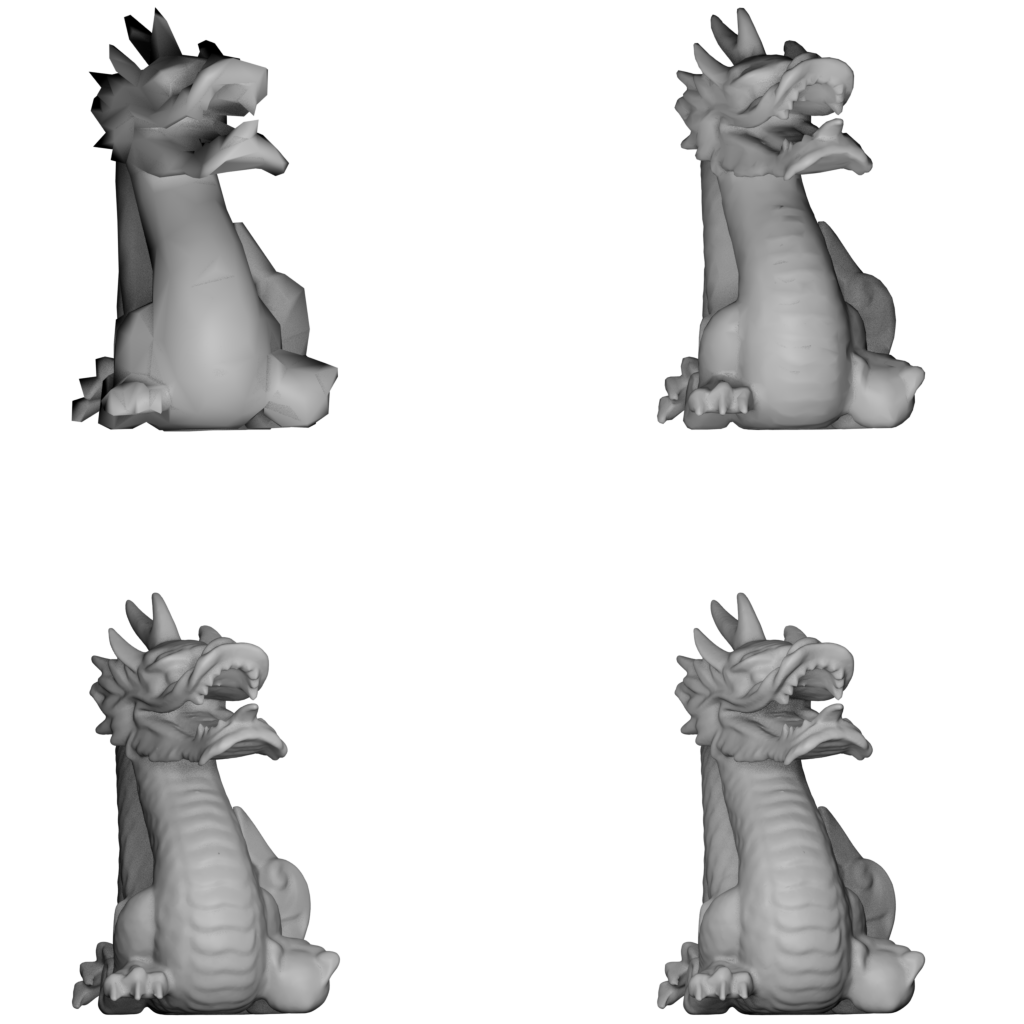
\includegraphics[width=\linewidth-130pt]{img/benchmark/smoki.png}}
  \caption{Model Stanford Dragon w czterech wariantach złożoności geometrycznej: lewa góra -- 1k, prawa góra -- 10k, lewy dół -- 100k, prawy dół -- 1M wierzchołków}
  \label{fig:stanford_dragon}
\end{figure}

\subsubsection{Środowisko testowe}
Pomiary zostały wykonane na komputerze wyposażonym w czterordzeniowy procesor o taktowaniu 2712 MHz z następującą hierarchią pamięci podręcznej:
\begin{itemize}
  \item L1 Dane: 32 KiB (x4)
  \item L1 Instrukcje kodu: 32 KiB (x4)
  \item L2 Połączony: 256 KiB (x4)
  \item L3 Połączony: 6144 KiB (x1)
\end{itemize}

\subsection{Wyniki pomiarów}

W tabeli \ref{tab:benchmark_results} przedstawiono zestawienie wyników pomiarów dla wszystkich wariantów modelu. Zmierzono trzy różne metryki czasowe: pełny czas ładowania (czas rzeczywisty, ang. \textit{wall clock time}), czas procesora CPU oraz czas samego parsowania pliku.

\begin{table}[h!]
  \centering
  \caption{Wyniki pomiarów wydajności ładowania modeli OBJ}
  \label{tab:benchmark_results}
  \begin{tabular}{|l|c|c|c|c|}
    \hline
    \textbf{Metryka}               & \textbf{1k} & \textbf{10k} & \textbf{100k} & \textbf{1M} \\
    \hline
    Pełne ładowanie (ms)           & 5,05        & 43,1         & 427           & 4290        \\
    \hline
    Czas CPU (ms)                  & 4,87        & 42,0         & 421           & 4282        \\
    \hline
    Tylko parsowanie (ms)          & 4,16        & 38,0         & 392           & 3927        \\
    \hline
    Odch. std. pełnego ład. (ms)   & 0,178       & 0,502        & 2,34          & 32,8        \\
    \hline
    Przepustowość (mln wierzch./s) & 1,19        & 1,39         & 1,40          & 1,38        \\
    \hline
  \end{tabular}
\end{table}

\subsubsection{Analiza skalowania czasowego}

Na rysunku \ref{fig:time_scaling} przedstawiono zależność czasu wykonania od rozmiaru modelu w skali podwójnie logarytmicznej. Liniowy charakter wykresu w tej skali potwierdza, że złożoność czasowa algorytmu jest proporcjonalna do liczby wierzchołków, tj. wynosi $O(n)$, gdzie $n$ oznacza liczbę wierzchołków.

\begin{figure}[h!]
  \centering
  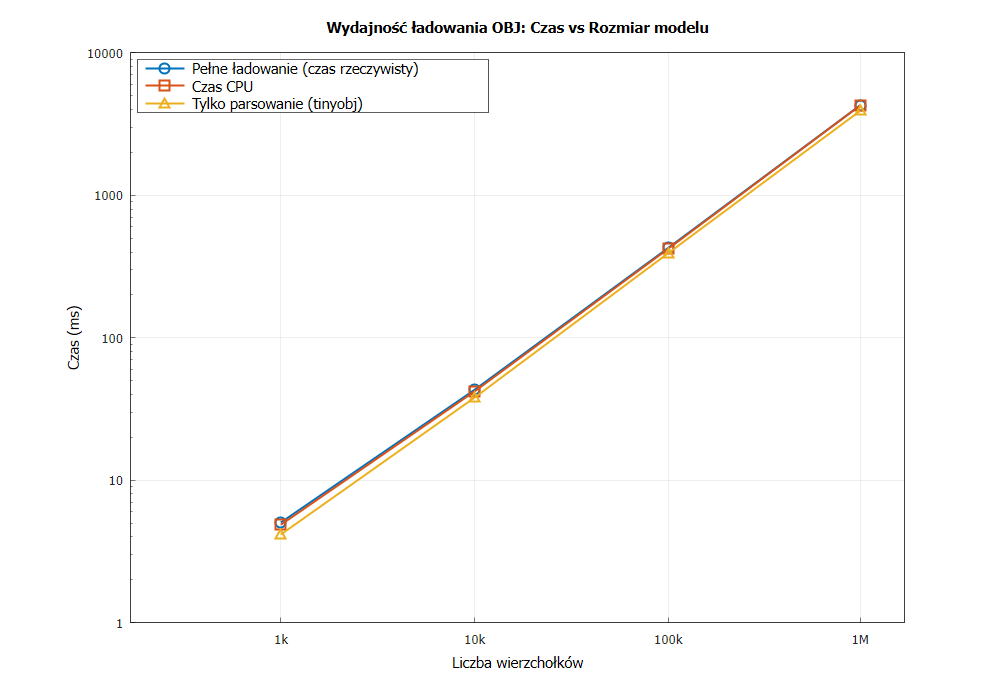
\includegraphics[width=\linewidth]{img/benchmark/benchmark_time_scaling.png}
  \caption{Zależność czasu ładowania od rozmiaru modelu (skala logarytmiczna)}
  \label{fig:time_scaling}
\end{figure}

Dla dziesięciokrotnego zwiększenia liczby wierzchołków czas wykonania rośnie około dziesięciokrotnie, co jest zgodne z oczekiwaniami dla algorytmu o liniowej złożoności obliczeniowej.

\subsubsection{Podział czasu wykonania}

Szczególnie istotna jest analiza podziału czasu między dwie główne fazy operacji: parsowanie pliku oraz obliczenia macierzy TBN. Na rysunku \ref{fig:time_breakdown} przedstawiono ten podział dla poszczególnych rozmiarów modeli.

\begin{figure}[h!]
  \centering
  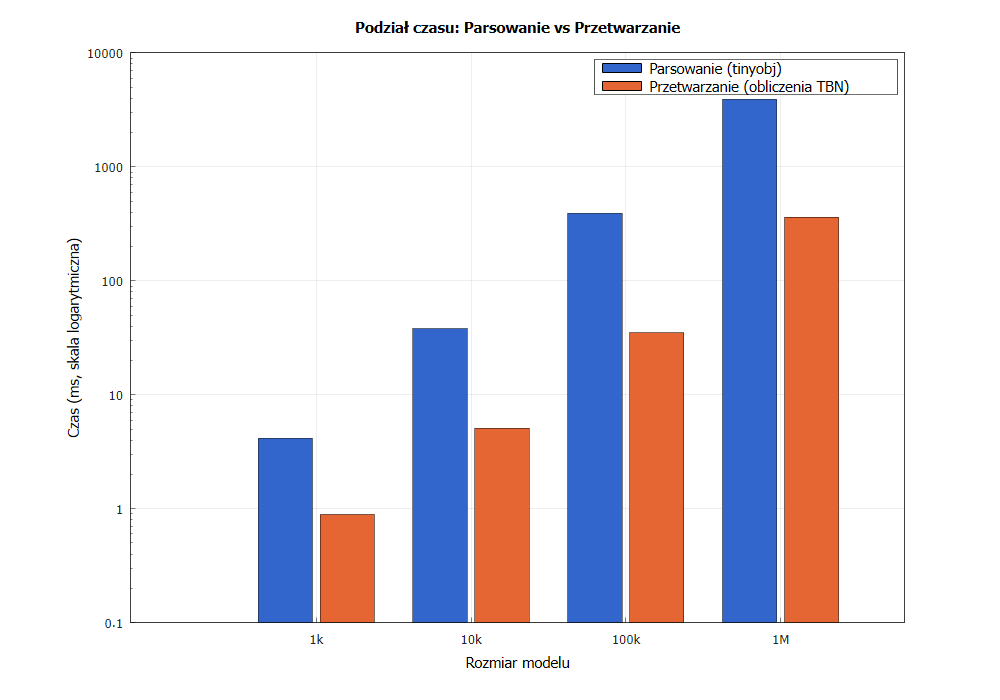
\includegraphics[width=\linewidth]{img/benchmark/benchmark_time_breakdown.png}
  \caption{Podział czasu: parsowanie pliku (niebieski) vs obliczenia TBN (pomarańczowy)}
  \label{fig:time_breakdown}
\end{figure}

Obliczenia macierzy TBN stanowią stały procent całkowitego czasu ładowania -- około 8-9\% dla wszystkich rozmiarów modeli. Oznacza to, że dominującym czynnikiem wpływającym na wydajność jest operacja parsowania pliku OBJ, która obejmuje odczyt z dysku oraz interpretację formatu tekstowego.

\subsubsection{Przepustowość}

Przepustowość operacji ładowania, wyrażona jako liczba przetworzonych wierzchołków na sekundę, utrzymuje się na stabilnym poziomie około 1,4 miliona wierzchołków na sekundę dla modeli powyżej 10 tysięcy wierzchołków (rysunek \ref{fig:throughput}). Niższa przepustowość dla najmniejszego modelu (1,19 mln wierzch./s) wynika z narzutu związanego z inicjalizacją operacji wejścia/wyjścia.

\begin{figure}[h!]
  \centering
  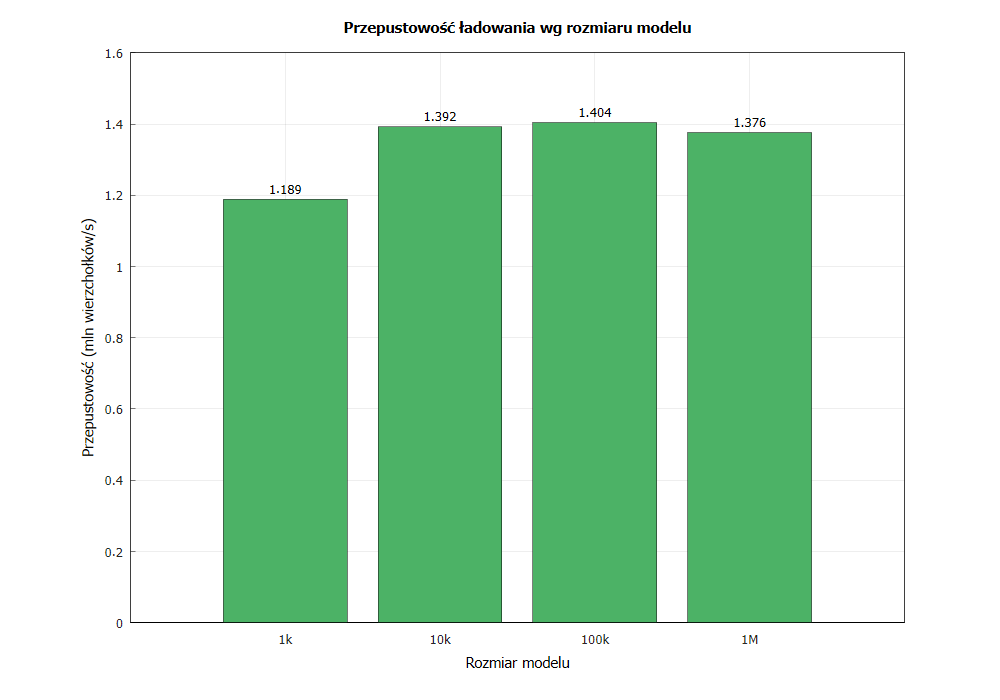
\includegraphics[width=\linewidth]{img/benchmark/benchmark_throughput.png}
  \caption{Przepustowość ładowania modeli OBJ}
  \label{fig:throughput}
\end{figure}

\subsubsection{Analiza stabilności pomiarów}

W celu oceny wiarygodności wyników obliczono współczynnik zmienności (CV, ang. \textit{Coefficient of Variation}), który jest miarą względnego rozproszenia wyników. Definiowany jest wzorem:
\begin{equation}
  CV = \frac{\sigma}{\mu} \cdot 100\%
\end{equation}
gdzie $\sigma$ oznacza odchylenie standardowe, a $\mu$ średnią arytmetyczną. Niższa wartość współczynnika zmienności świadczy o większej stabilności i powtarzalności pomiarów.

\begin{figure}[h!]
  \centering
  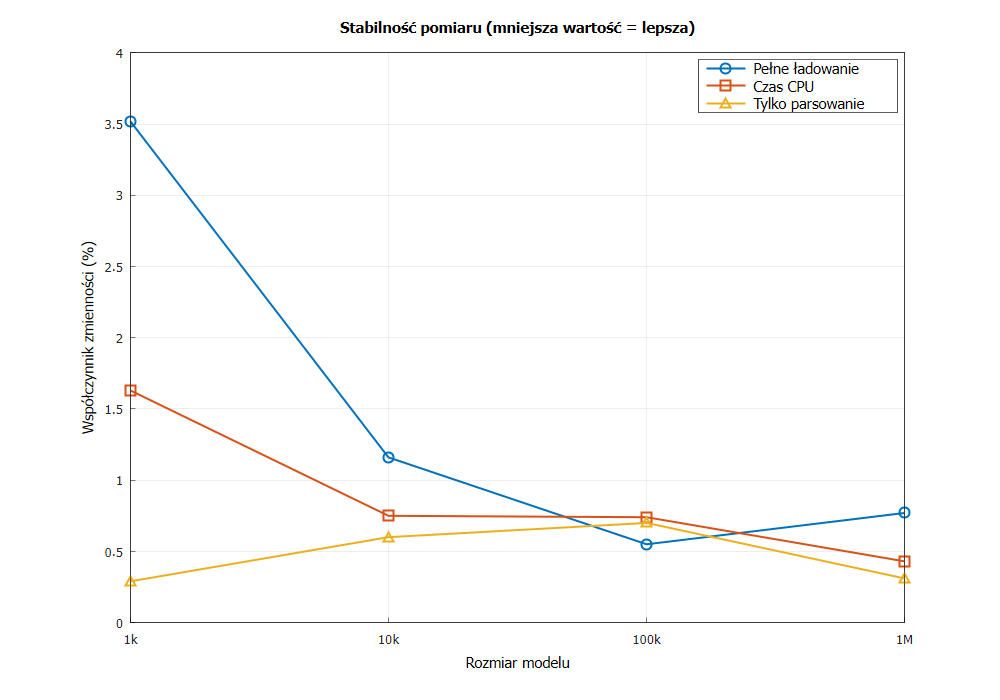
\includegraphics[width=\linewidth]{img/benchmark/benchmark_cv.png}
  \caption{Współczynnik zmienności pomiarów -- niższa wartość oznacza większą stabilność}
  \label{fig:cv}
\end{figure}

Jak widać na rysunku \ref{fig:cv}, współczynnik zmienności dla wszystkich pomiarów nie przekracza 4\%, przy czym dla większych modeli osiąga wartości poniżej 1\%. Świadczy to o wysokiej powtarzalności i wiarygodności przeprowadzonych pomiarów. Większa zmienność dla najmniejszego modelu (1k) wynika z proporcjonalnie większego wpływu szumów pomiarowych przy krótkim czasie wykonania.

\subsection{Wnioski z analizy wydajności}

Przeprowadzona analiza wydajności funkcji ładowania modeli OBJ pozwala sformułować następujące wnioski:

\begin{enumerate}
  \item \textbf{Liniowa złożoność} -- algorytm charakteryzuje się złożonością czasową $O(n)$, co oznacza, że czas ładowania rośnie proporcjonalnie do liczby wierzchołków w modelu.

  \item \textbf{Dominacja operacji I/O} -- parsowanie pliku tekstowego stanowi około 91-92\% całkowitego czasu ładowania. Optymalizacja tej fazy, np. poprzez użycie binarnego formatu plików, mogłaby znacząco poprawić wydajność.

  \item \textbf{Stabilna przepustowość} -- dla modeli powyżej 10 tysięcy wierzchołków przepustowość utrzymuje się na poziomie około 1,4 miliona wierzchołków na sekundę.

  \item \textbf{Wysoka powtarzalność} -- niski współczynnik zmienności (poniżej 1\% dla dużych modeli) świadczy o deterministycznym charakterze operacji i wiarygodności pomiarów.

  \item \textbf{Czas ładowania modeli produkcyjnych} -- dla typowego modelu o złożoności 100 tysięcy wierzchołków czas ładowania wynosi około 427 ms, co jest akceptowalne dla jednorazowej operacji inicjalizacji sceny.
\end{enumerate}

Uzyskane wyniki potwierdzają, że implementacja funkcji ładowania geometrii jest wydajna i skalowalna, spełniając wymagania aplikacji renderującej trójwymiarowe obiekty w czasie rzeczywistym.

